\documentclass[times, utf8, zavrsni, numeric]{fer}
\usepackage{booktabs}
\usepackage{indentfirst}

\tolerance=1
\emergencystretch=\maxdimen
\hyphenpenalty=10000
\hbadness=10000

\begin{document}
	
% TODO: Navedite broj rada.
\thesisnumber{4350}

% TODO: Navedite naslov rada.
\title{Razvoj podatkovnog sloja i aplikacijske logike za potrebe sustava elektroničkog učenja}

% TODO: Navedite vaše ime i prezime.
\author{Alen Murtić}

\maketitle

% Ispis stranice s napomenom o umetanju izvornika rada. Uklonite naredbu \izvornik ako želite izbaciti tu stranicu.
\izvornik

% Dodavanje zahvale ili prazne stranice. Ako ne želite dodati zahvalu, naredbu ostavite radi prazne stranice.
\zahvala{}

\tableofcontents

\chapter{Uvod}
Znanje i prenošenje znanja najznačajniji je faktor sve bržeg razvoja ljudske civilizacije, iako je često nailazilo na prepreke u širenju. Prije početka 20. stoljeća ponajveći je problem bila dostupnost znanja, a ta je prepreka postajala sve manja izumima kao što su tiskarski stroj, sveučilište te obveznim školstvom i masovnom proizvodnjom knjiga. Dostupnog znanja danas je minoran ili čak nepostojeći problem, no to je stvorilo novi izazov - odabir pravog načina učenja. Moderno elektroničko doba samo ga je još pojačalo jer je ogromna količina e-knjiga od korisnika udaljena na samo nekoliko klikova.
\par
Moderni svijet donosi golemu količinu dostupnih informacija što dovodi do toga da ljudska pažnja postaje sve neodređenija, a vrijeme fokusa sve kraće. Moderne generacije nemaju imperativ učenja kao njihovi preci, uglavnom zato što nikada nisu iskusile težinu ne-modernog života. Stoga se može dogoditi da čovjek željan znanja jednostavno odustane zbog ogromne količine mogućnosti, a posebno zbog činjenice se samo u ponekim školskim sustavima uči kako učiti.
\par
Shvativši da je znanje i prenošenje znanja izuzetno bitno te da je moderni svijet stvorio nove izazove učenju, postavlja se pitanje kako poboljšati njegovu kvalitetu? Odgovor je relativno jednostavan: pretvoriti učenje u nešto zanimljivo i jednostavno za korištenje, ali ipak izazovno i korisno - specijalizirane aplikacije, tj. sustave za elektroničko učenje.
\par
Ovaj završni rad opisat će što su sustavi za elektroničko učenje, što znači da je takav sustav inteligentan, neke od algoritama inteligencije, kako trebaju izgledati podatkovni i aplikacijski slojevi takvog sustava te objasniti što su oni uopće. U konačnici, temeljem principa navedenih u teoretskom dijelu, opisat će podatkovni i aplikacijski sloj sustava koji sam implementirao.
\par
Implementirani sustav je izgrađen za korištenje u edukacijske svrhe vezane uz predmete s matematičkom pozadinom (kao npr. Osnove elektrotehnike, Fizika, Matematika). Trenutno je ispunjen pitanjima iz područja diskretne matematike (skupovi, kombinatorika, osnove diskretne vjerojatnosti), no implementacija je skalabilna te ne postoji prepreka dodavanju novog znanja. Svrha implementacije je edukacija autora ovog završnog rada i demonstracija primjene teoretski opisanih elemenata u konkretnom sustavu za inteligentno učenje.

\chapter{Sustavi za elektroničko učenje}
Elektroničko učenje (e-učenje, \textit{e-learning}) je prijenos znanja ili obrazovnog programa putem elektroničkih uređaja poput računala ili mobitela. E-učenje može prenositi informacije i materijale, provjeravati znanje te biti korišteno za postupno upijanje novih činjenica baš kao na akademskim institucijama.\cite{derekstock} No, prednosti sustava za elektroničko učenje nad tradicionalnim akademskim institucijama su veća prostorna dostupnost (praktički jedini uvjet sudjelovanja je internetska povezanost) te brže ažuriranje gradiva novim informacijama u odnosu na spori obrazovni sustav.
\cite{eLearningNC}
\par
Sustavi za elektroničko učenje mogu biti dio nekog formalnog obrazovnog sustava ili samostalni. Moodle je primjer sustava za elektroničko učenje čiji je cilj obavljati samo dio obrazovanja, uglavnom provjere znanja i prenošenja informacija (materijala za učenje). Od korisnika se očekuje da sam proučava te materijale ili pohađa predavanja predmeta unesenog na sustav Moodle.\cite{moodle} Samostalni sustavi za elektroničko učenje trebali bi imati dostupne sve elemente učenja jer samo tako mogu osigurati kvalitetu. Eventualno može nedostajati formalna provjera znanja ako je sustav dizajniran tako da je postupak upijanja novih činjenica rigorozan u korištenju da ga korisnik ni u kojem slučaju ne može preskočiti ili ignorirati. 
\par
Neki od popularnih i besplatnih sustava za elektroničko učenje su Codecademy, Duolingo i Coursera. Coursera je zanimljiv koncept učenja koji na internet stranicu prenosi predmete stvarnih sveučilišta. Ona je za kranjeg korisnika samostalna, no stvaranje njezinog sadržaja nije.\cite{coursera} Duolingo je besplatan sustav za učenje stranih jezika u čijem održavanju uz zaposlenike sudjeluje i zajednica korisnika.\cite{duolingo} Na FER-u se uz Moodle također koriste AHyCo i Ferko.\cite{ferko}
\pagebreak
\section{Inteligentni sustavi za elektroničko učenje (ITS)}
Inteligentni sustavi za elektroničko učenje posebna su vrsta sustava za elektroničko učenje koja korisniku pruža reakcije ili upute prilagođene isključivo njemu. Cilj svakog ITS-a je smanjiti ovisnost korisnika sustava o ljudskim učiteljima. Za razliku od ljudi, elektronički sustavi se ne umaraju, ne stare, gotovo uvijek imaju vremena za učenika. Inteligentni sustavi za elektroničko učenje sadrže 3 glavne komponente: domenski model, korisnički model i model učenja te korisničko sučelje.\cite{aect}\cite{markurban} Naravno, inteligentni sustavi za elektroničko učenje također imaju svoje limite: kvalitetni su koliko je kvalitetan dizajner sustava, ne mogu pratiti fizičke reakcije korisnika i iskustveno zaključivati iz njih te, ipak, ne mogu biti potpuno individualni jer bi u tom slučaju količina praćenih podataka morala biti enormna.\cite{grubisic2006}

\subsection{Povijest ITS-a}

\subsubsection{Mehanički strojevi za učenje}
Ideja inteligentnih sustava za učenje nije nastala tek u 21. stoljeću, dapače, već u 17. st. dvojica od najvećih europskih matematičara, Blaise Pascal i Gottfried Wilhelm Leibniz razmatrali su koncepte zaključivanja uz pomoć strojeva.\cite{leibniz}\cite{pascal} Pravi zamah elektroničko učenje dobiva u 20. stoljeću.
\par
Prvi značajan korak prema učenju uz pomoć strojeva je napravio Sidney Leavitt Presley, profesor na Sveučilištu Ohio, koji je izumio stroj za samoocjenjivanje.\cite{pressey} Korisnik je odgovarao na pitanja s višestrukim izborom, stroj bi spremao odgovore te na kraju seta pitanja dao povratnu poruku o točnosti odgovora. Taj pristup koristi se i danas u većini akademskih sustava za ocjenjivanje jer je jednostavno prirodna opcija. Slika 2.1 prikazuje stroj za ocjenjivanje s gumbima za odabir točnog odgovora između ponuđenih.

\begin{figure}[htb]
	\centering
	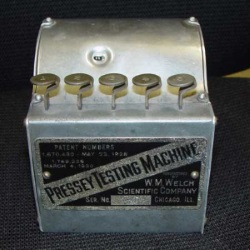
\includegraphics[]{img/pressey.jpg}
	\caption{Stroj za ocjenjivanje S. L. Presleyja\cite{presseymachinepic}}
	\label{fig:pressey}
\end{figure}

Iako su mehanički strojevi pružili kvalitetan početak ideje, jasno je da zbog nefleksibilnosti i skupoće izrade nikada nisu mogli prijeći fazu demonstracije. No, računalne aplikacije je lako umnožavati i mijenjati. Zato su one pogodne za razvoj sustava za učenje, ovog puta elektroničkih.

\subsubsection{Početak elektroničkih sustava za učenje}
U ranim godinama razvoja računala i računarstva napravljeni su mnogi koncepti bliskih tematika, npr. Turingov test, ideja umjetne inteligencije i strojnog učenja, no sustavi za učenje kao koncept kakav danas postoji je relativno zanemaren. Jedini važan napredak su definiranja gramatika u računarstvu, kao jednog od budućih načina parsiranja korisnikovih odgovora. No, dolaskom računala u širu upotrebu, u američkim školama se stvaraju CAI (\textit{Computer-Assisted instruction}) projekti s ciljem učenja programiranja. CAI sustav je takav da se korisniku prezentira neki materijal s uputom korištenja, nakon čega on na \textit{input-output} principu komunicira s računalom. Najbolji primjer nečega sličnog CAI sustavu u današnje vrijeme je Codecademy. U početku se CAI koristio u učionicama, a ne individualno, ali na sličnom principu korištenja.\cite{markurban} Na slici 2.2 nalazi se predviđena shema rada prilikom korištenja CAI sustava.

\begin{figure}[htb]
	\centering
	\includegraphics[]{img/CAI_shema.jpg}
	\caption{Shema rada pomoću CAI sustava\cite{caipic}}
	\label{fig:cai}
\end{figure}

\par
Velik korak za stvaranje ITS-a napravio je Jaime Carbonell koji je 1970. postavio tezu da "sustavi za učenje ne moraju biti samo alat, nego i učitelj".\cite{peters} U 1970.-ima je najpopularnije novo područje bila umjetna inteligencija temeljena na znanju. Najpoznatiji primjer takvog sustava je \textit{Dendral}, sustav zaključivanja o kemijskim strukturama korištenim u organskoj kemiji. Izgradnja složenijih sustava je bila lakša zbog poboljšanja brzine računala što je fokus rada konačno maknulo s tehnologije na tehniku. 
\par
Početkom 1980. umjetna inteligencija se pomiče k neuronskim mrežama i kognitivnoj psihologiji što otvara prostor razvoju sustava za elektroničko učenje zbog sličnih područja interesa. To dovodi do stvaranja koncepta ICAI-ja (\textit{Intelligent Computer Assisted Instruction}), vrste CAI sustava koji bi radio na principu prilagođenog posluživanja instrukcija. ICAI je jako blizu modernom konceptu ITS-a, jedina razlika između njih je što ICAI ne pokušava modelirati znanje korisnika.\cite{markurban}

\subsubsection{ITS u doba interneta i analize podataka}
Najvažniji korak za veću primjenu elektroničkog učenja je početak masovnog korištenja interneta. Internet je konačno omogućio neovisnost fizičkih pozicija korisnika sustava i kvalitete znanja koju mu sustav može pružiti. Slika 2.3 prikazuje broj korisnika mobilnog interneta centre u svijetu s ciljem podržavanja dojma sveprisutnosti interneta (osim, nažalost, u Africi). Slabost prijašnjih rješenja je bila u neadekvatnoj aktualizaciji sustava zbog činjenice da su se morali distribuirati na prijenosnim medijima. Nije slučajno da su svi sustavi koje sam na početku nabrojao internetske stranice.

\begin{figure}[htb]
	\centering
	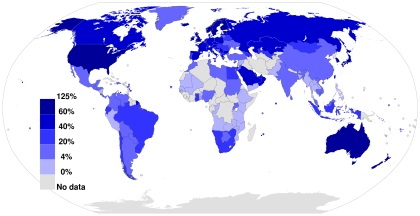
\includegraphics[]{img/internet.jpg}
	\caption{Broj korisnika mobilnog interneta prema državama u svijetu\cite{mobilenet}}
	\label{fig:internet}
\end{figure}

\par
Analiza podataka, je najveći korak u razvoju inteligencije ITS-a. Iako su principi analize podataka bili matematički postavljeni i prije 1990.-ih, rastom brzine računala, popularizacijom SQL-a i internet tražilica, analiza podataka doživjela je pravi \textit{boom} zadnjih 20-tak godina. Razlog tolike važnosti analize podataka u inteligenciji ITS-a je što kompleksnost procesa učenja (čime se bavi kognitivna psihologija), udaljenost sustava i potreba za prilagođenim (personaliziranim) sadržajem korisniku. Ti faktori se jednostavno ne mogu opisati malim brojem varijabli. Svaki učitelj kroz godine upoznaje nove učenike te nadopunjuje svoje znanje i tehniku, baš kao što bi ITS bio spreman za nadogradnju temeljem iskustva korištenja.
\par
Za razliku od UI čije rezultate velike tvrtke sigurno mogu naplatiti, razvoj sustava za inteligentno učenje je donedavno bio guran od strane akademske zajednice. Nove velike tehnološke tvrtke imaju potrebu educirati velik broj zaposlenika pa sustavi za učenje u današnje vrijeme konačno dobivaju zamah za napredak kao koncept, ali i u realizaciji.\cite{itspastpresentfuture}

\subsection{Komponente ITS-a}
Većina modernih ITS-ova dijeli se na 4 komponente rada: domenski i korisnički model, model učenja te korisničko sučelje. Tri prvonavedene komponente se nazivaju modeli zato što su pojednostavljena reprezentacija stvarnih pojava, koncepata i sl.\cite{aect} One nemaju nužno veze s modelom kao aplikacijskim slojem, iako se uglavnom oslanjaju na njega. Tri najvažnije komponente ITS-a i njihovo značenje mogu se vidjeti na slici 2.4.

\begin{figure}[htb]
\centering
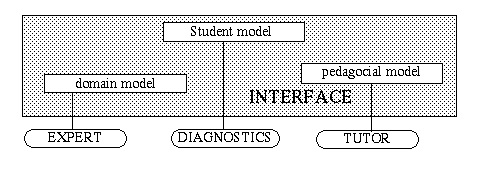
\includegraphics[]{img/ITS-components.jpg}
\caption{Komponente ITS-a\cite{itscomponents}}
\label{fig:its-comp}
\end{figure}

\subsubsection{Domenski model}
Domenski model je dio sustava čiji je smisao organizirati znanje u jedinice spremne za pohranu u bazu podataka.\cite{markurban} Svaki sustav osmišljava vlastitu podjelu znanja s obzirom na različitu širinu podjele i broj razina. U pravilu je neizbježna podjela na predmete u složenim sustavima i koncepte unutar predmeta, a na autorima i administratorima sustava je definirati više ili niže razine u odnosu na koncepte. Granulacija znanja je zato prilično kompliciran posao većoj količini autora, no budući da je kreiranje domenskog modela kreativan posao, u procesu zamišljanja treba sudjelovati što veći broj ljudi.
\par
Domenski model ne uključuje samo podjelu znanja, nego i pravila te strategije koje treba naučiti. Oni se mogu prikazati eksplicitno formulama i materijalima za učenje ili implicitno redoslijedom prikaza pitanja ili slično. Implicitno zadavanje pravila i strategija tipično je za formalne školske sustave zato što postoji određen redoslijed predavanja te nastavnici očekuju da učenici/studenti poznaju gradiva prethodnih predavanja. U sustavima za elektroničko učenje takav je pristup teže izvesti te se pravila i strategije najčešće zadaju eksplicitno u obliku najniže razine podjele u bazi podataka, iako korisnik uglavnom tu eksplicitnost ne vidi.
\par
Prilikom kreiranja domenskog modela važno je misliti na to da je takav model kvalitetna reprezentacija različitih vrsta znanja, da bude efikasan i razumljiv za kreiranje algoritama te da može odgovoriti na potrebe korisničkog modela.
\par
Tipični domenski model je kvalitetno organizirana baza podataka te pravilno uneseni podaci. Za sve iznad toga se brinu ostale komponente, počevši sa korisničkim modelom.

\subsubsection{Korisnički model}
Učenički, studentski ili jednostavno korisnički model je komponenta sustava čija se svrha većim dijelom preklapa s domenskom komponentom i modelom učenja. Razlog odvajanja korisničkog modela je bolja analiza znanja pojedinog korisnika. 
\par
Korisnički model su uglavnom algoritmi koji analiziraju točnost odgovora (te možda daju dodatne savjete korisniku) i algoritmi koji omogućuju prikaz analize odgovora korak po korak.\cite{markurban} Zbog relativno male opsežnosti, neki izvori zanemaruju korisnički model cijepajući njegove dijelove u domenski i model učenja. Algoritmi korisničkog modela opisani su u zasebnom poglavlju.

\subsubsection{Model učenja}
Nakon postavljanja domenskog i korisničkog modela, ostatak aplikacijske logike sadržan je u modelu učenja. Upravo je model učenja najbitniji dio inteligentnog sustava za elektroničko učenje jer on zamjenjuje ljudskog učitelja. Model učenja mora prikupljati podatke o korisniku, znati procijeniti znanje korisnika te isto prikazivati nekom opisnom ili grafičkom metodom.\cite{markurban}
\par
Ovoj komponenti pripadaju algoritmi koji na temelju rezultata prethodno navedenih evaluiraju znanje korisnika, algoritmi korisnikove navigacije sustavom te algoritmi posluživanja pitanja.
\par
Svrha modela učenja je praćenje korisnikova napretka u pojedinim konceptima/predmetima. Iako je na prvi pogled to relativno jednostavan problem, on jest takav za ljudskog učitelja, ali za računalo nije. Takvi problemi umjetne inteligencije (UI) nazivaju se UI-potpuni. Nakon što algoritmi procijene znanje korisnika, ono se treba prikazati nekim vizualnim načinom da korisnik bolje razumije što ne zna i zašto mu sustav postavlja neka pitanja.
\par
Model učenja je srž ITS-a te glavni odraz kvalitete pojedinog sustava. Čest način implementacije modela učenja je logičkim produkcijama koje dovode do zaključka je li korisnik nešto naučio ili ne.\cite{zhenzhai} Prednost takvog pristupa je formalna evaluacija korisnika i samog sustava, no nedostatak mu je nejasnost širem spektru administratora. Alternativni način je sustav bodovanja pojedinih pitanja, skupova pitanja i odnosa između koncepata koje korisnik treba savladati.

\subsubsection{Korisničko sučelje}
Korisničko sučelja je standardan element gotovo svake računalne aplikacije. Ono nužno ne mora biti grafičko, iako je takvo sigurno zanimljivije kranjem korisniku. Učenik treba vidjeti svoj trenutni napredak prikazan na jasan način, razumjeti na koji način sustav komunicira s njim i on sa sustavom te područje koje pitanja ispituju.

\subsection{Karakteristike dobrih sustava}
Nakon definiranja komponenata sustava za inteligentno učenje, potrebno je razmotriti koje karakteristike imaju kvalitetni sustavi za inteligentno učenje. Većina su obvezni dijelovi ITS-a te ih je baš zato važno navesti.

\subsubsection{Razrađena podjela znanja}
Iako se ovo čini kao očekivan uvjet iz  opisa domenskog modela, važno ga je ponoviti i u ovom dijelu. Ispravna podjela znanja omogućuje lakše i kvalitetnije projektiranje algoritama procjene korisnika.\cite{knowledgerep} Postoje dvije razine razrade podjele znanja: projektiranje sustava - odabir mogućih granula, povezanosti između njih i načina evaluacije znanja te projektiranje pitanja - punjenje sustava pitanjima i formulama za evaluaciju u skladu s dogovorenom podjelom.
\par
Granulacija podjele znanja je pitanje bez jednoznačnog odgovora, a s puno rizika. Ukoliko sustav ima premalo razina podjele, postoji rizik od nedovoljno dobrog praćenja korisnikova znanja, a sustav s previše razina podjele zahtijeva ogroman broj različitih pitanja da svaka od razina ima reprezentativni uzorak ocjene korisnika.
\par
Elegantno rješenje problema je određivanje srednje velikog broja granulacija (jasno, pojam srednjeg broja ovisi o opsegu domene za koju se ITS projektira), a onda između pojedinih granula uspostaviti različiti broj odnosa.\cite{sematicknowledge} Na taj način sam i ja riješio problem u svojoj implementaciji. Slika 2.5 ilustrira podjelu ljudskog znanja.

\begin{figure}[htb]
	\centering
	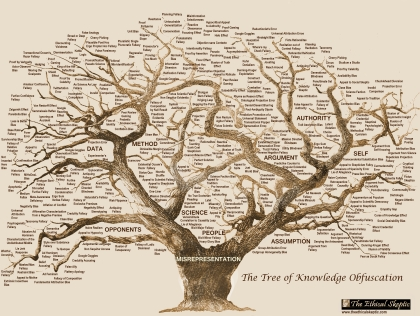
\includegraphics[]{img/drvo.jpg}
	\caption{Ilustracija: drvo znanja\cite{drvoznanja}}
	\label{fig:drvo}
\end{figure}

\subsubsection{Materijali za učenje}
Svaki sustav čiji je cilj biti samostalan trebao bi sadržavati materijale za učenje poput e-knjiga ili uputa koju bi literaturu korisnik morao proučiti prije odgovaranja. Samo takav pristup sa sigurnošću korisniku omogućava točnost znanja ili, ako se kasnije utvrdi pogreška u materijalima, referencu na pogrešku. Ukoliko sustav korisniku nudi samo provjeru znanja s objašnjenjima za pojedino pitanje, postoji velik rizik da korisnik neće dovoljno dobro razumjeti povezanost činjenica koje sustav ispituje.

\subsubsection{Parametrizirana pitanja}
Zamislite slučaj u kojem ITS služi za formalnu provjeru znanja na fakultetu čiji studenti imaju organizirane forume na kojima dijele zadatke. Nerealno je očekivati da može postojati više od 20 pitanja neke domene, a postoji preko 500 studenata u generaciji. Kako osigurati adekvatnost provjere? Odgovor je jednostavan: parametrizacijom pitanja.
\par
Parametriziranje pitanja je postupak kojim se numerička (moguće i na tekstualnim, ali teže) pitanja u ITS zapisuju u obliku formula za evaluaciju. Korisnicima se prikazuju njihove vlastite vrijednosti pojedinih parametara, a točnost odgovora evaluira se formulom. Takav pristup ne samo da omogućuje jedinstvene vrijednosti različitim korisnicima, nego i različite vrijednosti istim korisnicima. Ukoliko neki korisnik želi ili mora više puta rješavati pitanja nekog koncepta, mogu mu se servirati jedinstvene vrijednosti parametara svaki put kada otvara to pitanje. Jedan od načina ostvarivanja parametrizacije pitanja je spremanje formule kao odgovora te popisivanja vrijednosti parametara i njihovih ograničenja (npr. imaginarni dio broja mora biti različit od 0, apsolutna vrijednost mora biti > 0 i sl.).

\subsubsection{Praćenje tipkanja i reakcija lica korisnika}
Jedna od najvažnijih karakteristika dobrog učitelja je uočavanje učenikovih reakcija, čitanje fizičkih znakova te zaključivanje iz toga. Najveći nedostatak sustava za učenje, kao i svake druge vrste udaljenog učenja, je fizička udaljenost učenika i učitelja. Stoga, elektronički sustavi za učenje moraju naći drukčije načine praćenja reakcija korisnika.
\par
Dva najrazvijenija načina su praćenje tipkanja i izraza lica. Rastom količine prostora na tvrdim diskovima i brzine računala, stvorila se mogućnost praćenja naizgled trivijalnih detalja kao što je obrazac tipkanja pojedine osobe. Neki izvori kažu da svaka osoba ima jedinstven obrazac tipkanja, baš kao otisak prsta. Zato bi bilo važno pratiti u kojim je situacijama korisnik ubrzan, o kojim pitanjima dulje razmišlja te je li mijenjao neki odgovor.
\par
Praćenje izraza lica također je postalo moguće rastom brzine računala, njihove procesorske i grafičke snage te razvojem računalnog vida kao područja računarstva. Ideja takvog pristupa je aproksimirati ljudskog učitelja, no to je vrlo složen i težak posao. Nedostatak takvog pristupa je što svaki korisnik mora imati neki oblik web kamere.
\par
Oba dijela su dio najnaprednijih sustava s velikim budžetima za izradu zato što ih je složeno implementirati. 

\subsubsection{Prilagođene reakcije}
Neizostavna komponenta sustava za inteligentno učenje su reakcije (engl. feedback) temeljene na znanju korisnika.\cite{feedback} Jasno je da računalne aplikacije ipak ne mogu biti jedinstvene kao ljudski učitelji. Svejedno, reakcije sustava moraju biti kvalitetne i prilagođene pojedinom korisniku da bi ITS imao smisla. Postižu se analizom odgovora korisnika i njegova načina odgovaranja (trajanjem računanja, brojem izmjena odgovora prije potvrde i sl.) te dobrim projektiranjem sustava (postojanjem reakcije za svaku kombinaciju razine znanja).\cite{aect}
\par
Određivanje kada korisniku treba dati uputu (engl. hint) ako je zapeo na nekom zadatku je pitanje bez jednoznačnog odgovora, uostalom, kao i ljudskim učiteljima. S jedne strane učitelj mora znati detektirati kada je njegov učenik iscrpio sve mogućnosti, a s druge je jasno da otvoreno pitanje u sustavu za elektroničko učenje može značiti to da je korisnik jednostavno otišao od svojeg računala. Dva rješenja koja se nameću su pamćenje mogućih pogrešnih kombinacija parametara i broja pokušaja te dopuštanje korisniku da zatraži uputu ako sam shvaća da nema ideju. Nedostatak prvog rješenja je moguća prevelika nepotrebna složenost, a drugog to što umorni korisnici ponekad odustaju prerano.
\par
Alternativni način rješavanja reakcija je jednostavno pustiti korisnika da odgovori krivo i dati mu uputu nakon što završi provjeru.

\subsubsection{Sigurnost}
Sigurnost je jako važan element svakog sustava, a to se ističe u dva aspekta: zaštita osobnih podataka i sprječavanje lažnog predstavljanja. Iako osobni podaci u ITS-u gotovo sigurno ne bi trebali sadržavati osjetljive informacije, važno ih je zaštiti nekim sustavom lozinki.\cite{security}
\par
Sprječavanje lažnog predstavljanja je puno zanimljiviji problem. Ukoliko sustav ima ugrađeno praćenje tipkanja korisnika ili izraza lica, prilično je očito da bi takav pristup minimizirao rizik lažnog predstavljanja. No, što ako nema? Alternativna opcija je formalno rješavanje ispita ITS-a uz prisustvo administratora što vodi do gotovo potpunog eliminiranja samostalnog učenja. Tako da niti to nije najbolje rješenje. Koje onda jest? Zapravo ga i nema, sustav nažalost mora vjerovati korisniku ako ne želi implementirati skupe tehnologije praćenja tipkanja ili računalnog vida.

\subsubsection{Kvalitetni algoritmi}
Kvalitetni algoritmi su nešto što se gotovo podrazumijeva ukoliko želimo kvalitetan sustav. Sljedeća lekcija govori više o algoritmima sustava za elektroničko učenje, no bilo ih je važno navesti i u ovoj.

\subsubsection{Dizajn sučelja}
Posljednja, ali ne i najmanje važna karakteristika ITS-a je dizajn grafičkog korisničkog sučelja. To nije važno samo za ITS, nego i za svaku drugu računalnu aplikaciju jer loše sučelje odbija korisnike više nego bilo što drugo. Prilično je teško točno definirati što je kvalitetno grafičko korisničko sučelje, no ono bi sigurno moralo imati sljedeće karakteristike: intuitivnost rasporeda kontrola, lakoća upravljanja (brzina, dosljednost, dozvole promjena kontrola), ugodan izgled (boje, fontovi, izbjegavanje neugodnih efekata i promjena boja) te prikladan prikaz informacija.
\par
Korisničko sučelje ITS-a također bi se trebao držati nekih principa jedinstvenih za to područje. Tri najvažnija principa su: mogućnost traženja upute (također su opcije gumb za odustajanje ili ispis odgovora), konzistentnost znakovlja (npr. cos ili csin za kosinus, točka ili zarez kao decimalna oznaka) te prikaz napretka u pojedinoj granulaciji znanja.\cite{interface}

\subsection{Algoritmi sustava za inteligentno učenje}

Najprije smo saznali koji su dijelovi inteligentnog sustava za elektroničko učenje te koje principe moramo slijediti prilikom implementacije jednog takvog sustava, no sljedeće je pitanje što sve treba implementirati da bi sustav bio inteligentan. Najbolji odgovor je odrediti koje sve algoritme ITS treba imati, tj. koje bi poslove njegovi najvažniji algoritmi trebali odrađivati.

\subsubsection{Odabir pitanja}
Vjerojatno najznačajniji algoritam sustava za inteligentno učenje je algoritam odabira pitanja. Upravo je on najvažniji element umjetne inteligencije ITS-a.\cite{aect} Može biti oblikovan na različite načine, no dva su najčešća: logičkim produkcijama koje nadopunjuju produkcije procjena korisnikova znanja ili samostalan programski odabir. Prednost logičkih produkcija je konzistentnost tehnologija koje sustav koristi, no značajni nedostaci su im ovisnost o apsolutnoj točnosti produkcija evaluacije znanja te potreba da autor pitanja sastavlja algoritam. Zato se često koristi druga metoda.
\par
Programski odabir pitanja definiran je na razini sustava, a radi na principu procjene korisnikova znanja pojedine granulacije i odnosa između njih te odabira podskupa pitanja iz skupa onih koja je moguće postaviti. Pitanja se odabiru tako da se uračuna korisnikovo znanje, zahtjevnost i složenost pojedinog pitanja, što bi korisnik naučio ili dokazao točnim odgovorom na to pitanje te ukupna složenost provjere koja sadrži ta pitanja.

\subsubsection{Generiranje parametara}
Nakon što je sustav odabrao pitanja koja će postaviti, mora odrediti konkretne parametre svakog od njih. Algoritam generiranja parametara ih može generirati iz neke mape mogućih slučajeva ili nasumičnom generacijom uz određene uvjete. Uvjeti generiranja parametara važan su element tog postupka kako se ne bi dogodilo da se nekom korisniku postavi pitanje u čijem je rješenju npr. greška dijeljenja s 0. Ukoliko se unutar sustava dobro definiraju ograničenja, generiranje parametara postaje posao poziva funkcija slučajnih brojeva dok se ne zadovolje ograničenja.

\subsubsection{Evaluacija odgovora}
U dobro projektiranom sustavu evaluacija odgovora svodi se na procjenu točnosti formule zapisane u bazi podataka za određene parametre. U formuli se parametri promijene u stvarne brojeve te ona prolazi provjeru jednakosti +/- n\% s korisnikovim rješenjem.

\subsubsection{Procjena znanja}
Algoritmi procjene znanja mogu se temeljiti na različitim pogledima na korisnikov odgovor. Neki od najzanimljivijih faktora je li ili nije korisnik nešto naučio su točnost pitanja koja pripadaju nekoj granulaciji, odnosi između znanja, složenost zadatka u odnosu na ostale zadatke koje je korisnik riješio, koliko je vremena prošlo od zadnjeg ispitivanja pojedine granulacije, težina tog pitanja drugim korisnicima koji su došli do njega i koliko je dugo korisnik rješavao to pitanje.
\par
U praksi je algoritam procjene znanja najkreativniji dio sustava za inteligentno učenje jer su mu jedina ograničenja da se mora izvesti u nekom razumnom vremenu i da, naravno, sustav pamti tražene vrijednosti.
\par
Algoritam procjene znanja također može biti zapisan logički ili programski, u njegovom slučaju je logički češća pojava. Takav algoritam na temelju zapisanih produkcija donosi odluke koliko neke granulacije je korisnik naučio. Za svaki njezin dio se izbacuje vrijednost 1 (naučeno) ili 0 (nenaučeno). Programska alternativa može raditi isti taj posao drukčijom tehnologijom, oslanjati se na praćenje korisnika za \textit{data mining} ili donositi odluke na nekom trećem principu. Prednost programskog nad logičkim izračunavanjem je što programski u pravilu može elegantnije doći do neke ocjene i što ne mora ovisiti o konkretnim granulacijama. Slika 2.6 prikazuje općenitu shemu redoslijeda u logičkoj evaluaciji.

\begin{figure}[htb]
	\centering
	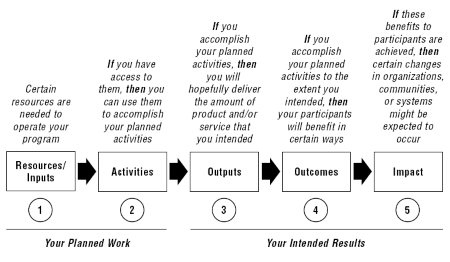
\includegraphics[]{img/logic.jpg}
	\caption{Općenita shema logičke evaluacije\cite{logicalevalpic}}
	\label{fig:logic_eval}
\end{figure}

\subsection{Poznati sustavi}

Znamo što sve treba napraviti prilikom dizajniranja sustava za inteligentno učenje, no nismo pogledali što su pametni ljudi prije nas radili u tom pogledu. A radili su puno, stoga bi bilo šteta propustiti izvući znanje i iskustva njihovih sustava u cilju dizajniranja jednog kvalitetnog ITS-a. Čak i neinteligentni sustavi mogu ponuditi korisne zaključke, možda čak i jasnije nego inteligentni. Zašto? Zato što su konceptualno relativno jednostavni te kod njih lakše možemo uočiti neke probleme.
\par
Bitno je naglasiti da nisu svi sustavi u ovom dijelu samo pitalice, već sadrže neke slobodnije poglede na učenje jer različiti ljudi uče na različite načine. Učiti se može vizualnom tehnikom, slušanjem, igrom, ponavljanjem / čitanjem naglas, rješavanjem zadataka, gradnjom rješenja itd. Zato bi bilo kontraproduktivno da svaki sustav za učenje ima oblik pitalice.

\subsubsection{Neinteligentni sustavi}

Duolingo je sustav za učenje jezika u čijoj izradi mogu sudjelovati i korisnici. Princip rada Duolinga je da korisnik odabere svoj materinji (ili dobro poznati jezik) te dobije ponudu jezika za koje postoji "tečaj" uz pomoć njegova materinjeg jezika.\cite{duolingo} Pitanja mogu biti dopunjavanje, prevođenje ili pitanje s odabirom od ponuđenih odgovora. Sustav je neinteligentan osim u dva pogleda: znanje nekog područja zastarjeva ukoliko korisnik nije dugo odgovarao na pitanja tog područja te sustav odabire područje s najmanjom vrijednosti znanja ukoliko korisnik odabere opciju "pojačavanja znanja" (engl. strengthen skills). Na slici 2.7 može se vidjeti prepoznavanje pogreške tipkanja u sustavu Duolingo.

\begin{figure}[htb]
	\centering
	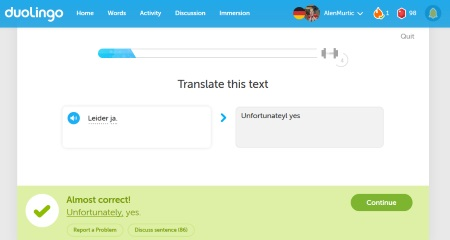
\includegraphics[]{img/duolingo.jpg}
	\caption{Inteligentni aspekt sustava Duolingo: prepoznavanje "tipfelera"}
	\label{fig:duolingo}
\end{figure}

\par
Coursera je internetska stranica koja sadržava kolegije najpoznatijih svjetskih sveučilišta s ciljem smanjivanja ovisnosti fizičke pozicije ljudi i njihovih mogućnosti učenja. Sadrži besplatne i plaćene tečajeve čije materijale korisnik može (i mora) proučavati, odgovarati na pitanja te na kraju dobiti potvrdu svojeg znanja.\cite{coursera} Jasno je da položiti neki tečaj na Courseri nije jednakovrijedno kao završiti kolegij na fakultetu, no ukoliko korisnik ima stvarnu volju za učenjem, količina stečenog znanja može biti jednaka. Iako su materijali velikog broja fakulteta (pogotovo tehničkih) javno dostupni, Coursera eliminira potrebu za iscrpnom pretragom materijala i stavlja fokus na učenje.
\par
Urban Jungle je simulacija vožnje koju su izradili Autoklub i Udruga darovitih informatičara Rijeka da bi mladima olakšali polaganje vozačkog ispita.\cite{urbanjungle} Korisnik  može voziti virtualni automobil kao i u sličnim računalnim igrama, no Urban Jungle ima edukativnu svrhu jer za uspješno "igranje" korisnik mora paziti na stvarna prometna pravila. Odličan je primjer da računalni sustav namijenjen za učenje ne mora nužno biti samo niz pitanja i odgovora. Slika 2.8 prikazuje ekran tijekom simulacije vožnje u aplikaciji Urban Jungle. 

\begin{figure}[htb]
	\centering
	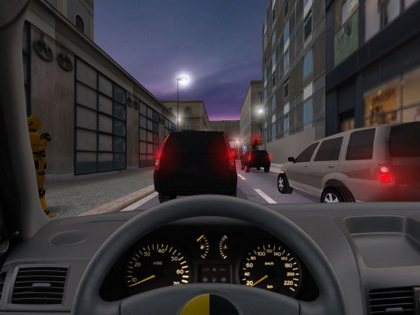
\includegraphics[]{img/urbjng.jpg}
	\caption{Slika ekrana prilikom vožnje u Urban Jungle edukativnoj igri\cite{urbanjungpic}}
	\label{fig:urbjng}
\end{figure}

\par
Moodle je vrlo popularan akademski sustav za učenje koji omogućava neke koncepte ITS-a (parametrizirana pitanja, interaktivno sučelje), no nije ITS jer ne sadrži inteligentno odlučivanje.\cite{moodle} Sustav Moodle gotovo uvijek funkcionira kao podrška formalnom sustavu učenja zato što omogućava planere, kalendare, obavijesti korisnicima i sl. Moodle može biti osnova za izgradnju drugog sustava za učenje, kao što je slučaj s CARNet-ovim sustavom Merlin. Moodle je aplikacija otvorenog koda te ju je zato moguće lako prilagođavati. Sustav Ferko razvijen na Fakultetu elektrotehnike i računarstva ima sličnu domenu primjene kao Moodle. Slika 2.9 prikazuje logo sustava Moodle, a slika 2.10 sustava Merlin.

\begin{figure}[htb]
	\centering
	
\includegraphics[]{img/moodle.jpg}
	\caption{Logo sustava Moodle\cite{moodlelogopic}}
	\label{fig:moodle}
\end{figure}

\begin{figure}[htb]
	\centering
	
\includegraphics[]{img/merlin.jpg}
	\caption{Logo sustava Merlin temeljenog na Moodleu\cite{merlinpic}}
	\label{fig:merlin}
\end{figure}

\subsubsection{Inteligentni sustavi}
Postoje mnogi sustavi za inteligentno učenje koji rade na principu pitalica te sam zato odabrao najzanimljivije primjere ITS-a koji možda i ne slijede dosad navedeni obrazac, no svejedno pripadaju skupini sustava za inteligentno učenje.
\par
Why2-Atlas je ITS koji uči korisnika koncepte kvalitativne fizike tako da traži od njega da napiše nekoliko rečenica o određenom pojmu te abduktivnom sintaktičkom analizom pokušava dokučiti znanje korisnika. Takav proces može se odvijati u nekoliko iteracija dok sustav ne odredi znanje korisnika te ga uputi na točno rješenje ukoliko je u krivu.\cite{why2atlas}
\par
AutoTutor je sustav za inteligentno učenje razvijen na Arizona State sveučilištu koji razgovara s korisnikom prirodnim jezikom. Princip rada AutoTutora je parsiranje govora na sličan način na koji se prevode programski jezici.\cite{autotutor} Prikaz sučelja sustava AutoTutor nalazi se na slici 2.11.

\begin{figure}[htb]
	\centering
	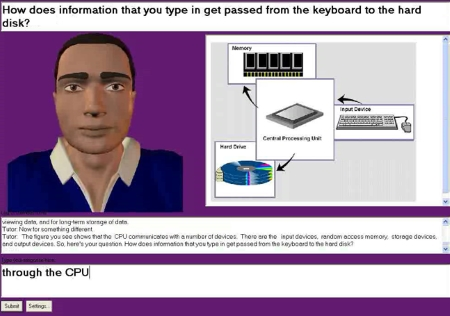
\includegraphics[]{img/autotutor.jpg}
	\caption{Sučelje razgovora sustava AutoTutor\cite{autotutorpic}}
	\label{fig:autotutor}
\end{figure}

\par
ActiveMath je ITS vrlo sličan prototipskom pogledu na sustave za inteligentno učenje. To je sustav za dodatno podučavanje matematike u školama ili učenje na daljinu. ActiveMath je internetska stranica na kojoj pored sustava za učenje postoje i materijali koji pokrivaju gradivo. Kvaliteta ActiveMath ITS-a je u tome što ga autori prilagođavaju s obzirom na empirijske rezultate kako su korisnici učili.\cite{activemath} Slika 2.12 prikazuje korisničko sučelje sustava ActiveMath.

\begin{figure}[htb]
	\centering
	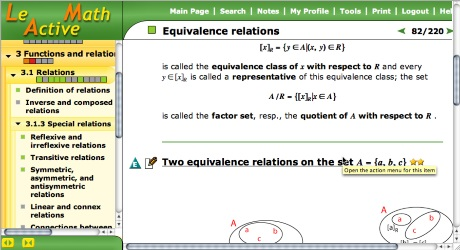
\includegraphics[]{img/activemath.jpg}
	\caption{Slika ekrana ActiveMath sustava\cite{activemathpic}}
	\label{fig:activemath}
\end{figure}


\par
Igre s prilagodljivom umjetnom inteligencijom (adaptive AI) nisu namijenjene za učenje, no svejedno imaju mnogo dodirnih točaka sa sustavima za inteligentno učenje. Ideja takvih igara je uočiti najčešće igračeve obrasce ponašanja te nove protivnike stvoriti takvima da igrač mora odabrati drukčiju strategiju. Mnogo računalnih igara tvrde da imaju prilagodljivu UI, no zasad taj koncept nije posebno dobro implementiran. Nogometne simulacije i strateške igre u stvarnom vremenu (engl. RTS) najviše reklamiraju takvu UI, no iskustva korisnika kažu da je UI u njima lošija nego prije desetak godina.\cite{adaptiveai}

\pagebreak

\subsection{Nedostaci ITS-a}

\subsubsection{Podučavanje i inteligencija}
Metode uspješnog podučavanja su očito najveći izazov svakog elektroničkog sustava za učenje. Iako neki izvori navode da kod problema koji se mogu rastaviti na sitne korake elektronički sustavi i ljudski učitelji imaju sličan rezultat usvojenosti gradiva kod učenika, podučavanje nije samo prenošenje znanja. Ono uključuje i metode usvajanja gradiva, procjene korisnikova znanja te oblikovanja odgovarajućih procesa učenja.
\par
Ponajveći problem metoda podučavanja i inteligencije ITS-a je što (zasad) nemaju pitanja "zašto?", "kako?" na korisnikov odgovor te kao takvi ne mogu dovoljno dobro procijeniti je li korisnik samo naučio "kuharicu", tj. formule za rješavanje zadataka. Jasno da sustav može pitati ta pitanja, no ona su svejedno organizirana po nekom predviđenom obrascu. Možda je nekada uputno pitati korisnika neka pitanja koja navodno zna kako bi bili sigurni da nešto stvarno razumije. Tu do izražaja dolazi intuicija učitelja koju sustavi (zasad) nemaju. Intuiciju donosi umjetna inteligencija temeljena na potpornom učenju, a ona je prilično različita od produkcijske umjetne inteligencije koju ITS koristi za definiranje je li korisnik nešto naučio.
\par
Drugi problem podučavanja je koliko korisniku sustav treba pomagati u rješavanju zadataka. Teza takve kritike je da korisnik jednostavno ne nauči dovoljno ukoliko mu sustav ponudi rješenje, da je takvo učenje previše površno. Osobno se slažem s tim pogledom i mislim da bi korisniku bilo korisnije prikazati bitnije upute tek nakon završene provjere, a onda ga manje kažnjavati (u dugoročnom pogledu) za krive odgovore.\cite{limitations}
\par
Naravno da je i problem ITS-a što autori pitanja jednostavno moraju odlično razumijevati tehničku pozadinu sustava (smisao pojedine granulacije, veze između granula) te ako ne razumiju ili sustav nije dovoljno dobro projektiran, u sustavu bi moglo doći do problema u definiranju korisnikova znanja ili otvaranju pitanja. Rizik površnog učenja je u takvim situacijama značajno veći.

\subsubsection{Cijena izrade}
Nadam se da je čitatelju jasno iz prethodnog dijela završnog rada da je izrada kvalitetnog ITS-a vrlo složen posao. Čak ne niti toliko težak, koliko opsežan. Problem izrade ITS-a je nužna bliska suradnja između računalnih stručnjaka i učitelja domene primjene. Velik broj ljudi koji moraju raditi istovremeno znači da je potreban velik broj radnih sati, što znači da ih treba platiti. Ukoliko vlasnik sustava ne očekuje da će mu ITS značajno povećati broj korisnika, logično je postaviti pitanje opravdanosti investicije. Pogotovo imajući u vidu cijenu održavanja sustava i rizik pogreške u sustavu. Zato je dosad ITS-ove uglavnom razvijala akademska zajednica. Na slici 2.13 može se vidjeti ilustracija timskog rada potrebnog za projektiranje kvalitetnog sustava za učenje.

\begin{figure}[htb]
	\centering
	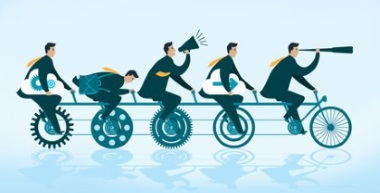
\includegraphics[]{img/teamwork.jpg}
	\caption{Ilustracija timskog rada potrebnog za dobar ITS\cite{teamwork}}
	\label{fig:teamwork}
\end{figure}

\par
Drugi problem kod cijene izrade je kompleksnost sustava. Sustav za učenje jednostavno mora biti efikasan i brz, a sustav koji prati sve faktore to jednostavno ne može biti. Inženjeri koji ga projektiraju moraju napraviti \textit{trade-off} između brzine i kvalitete sustava.
\par
Cijena izrade zapravo i nije nedostatak, njezin problem je što se mora platiti prije nego što sustav počne s radom. Dugoročno je ITS jeftiniji nego financiranje prostora, profesora, opreme učenika i sličnih elemenata tradicionalnog edukacijskog procesa.\cite{limitations}

\chapter{Slojevi aplikacija}
Sve kvalitetno oblikovane moderne aplikacije moraju sadržavati nekoliko slojeva rada. Slojevita arhitektura omogućuje sigurno zadržavanje dva najvažnija logička načela dobrog oblikovanja: nadogradnju bez promjene i načelo jedinstvene ovisnosti. Takav pristup intervencije u kod aplikacije čini lakšim. Arhitektura koju koristim je MVC (Model - View - Controller). Prevedeno na hrvatski, model je podatkovni sloj, controller je aplikacijska logika, a view pogled. Najveća prednost ovakvog pristupa je jednostavna i intuitivna višeplatformska modularnost - podatkovni sloj je zajednički za sve platforme, aplikacijsku logiku može koristiti više različitih platformi (npr. kod pisan u Javi za Android i web aplikacije ili C\# za Windows 10 i web), a svaka platforma određuje svoje korisničko sučelje, tj. pogled.\cite{mvc} Slika 3.1 prikazuje dijagram komunikacija u MVC modelu.

\begin{figure}[htb]
	\centering
	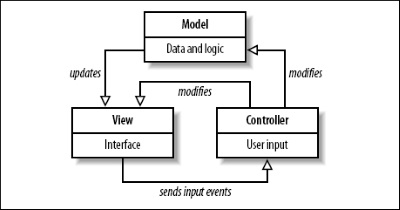
\includegraphics[]{img/mvc.jpg}
	\caption{Komunikacija u MVC modelu\cite{mvccommpic}}
	\label{fig:mvc}
\end{figure}

\par
Podatkovni sloj je sloj pohrane, dohvata i ažuriranja podataka, gotovo uvijek izveden u obliku baze podataka te ponekad pripadnih tehnologija kao npr. Entity Framework koji mapira objekte i bazu podataka. Podaci spremljeni u podatkovnom sloju moraju biti u \textit{display-neutral} obliku, što znači da bez daljnje obrade nisu previše pogodni za sami prikaz. Cilj takvog pristupa spremanja podataka je imati bazu u prve tri normalne forme te posljedično očuvati performanse baze na visokoj razini čak i uz veću količinu podataka spremljenih u nju. Podatkovni sloj implementiran u ovom završnom radu je SQL baza podataka te Entity Framework.
\par
Aplikacijska logika je sloj upravljanja korisničkim zahtjevima, a radi kao poveznica između prikaza i podatkovnog sloja. Aplikacijska logika prima naredbe koje je korisnik zadao na pogledu, zatim provodi neke operacije nad modelom, uzima podatke iz modela te ih u \textit{display-neutral} obliku šalje pogledu. Ona je uglavnom implementirana kao nekoliko slojeva različitih poslova, npr. \textit{utlity} sloj rada s bazom, sloj koji prima podatke od pogleda te algoritamski sloj koji provodi operacije. U ovom završnom radu aplikacijska logika će upravo raditi na taj način: statičke klase rada s bazom, klase algoritama odabira pitanja te klase koje primaju pozive operacija s korisničkog sučelja.
\par
Pogled, tj. korisničko sučelje je način na koji se aplikacija prezentira kranjem korisniku te način na koji je on koristi. Njegov je cilj rada obraditi podatke tako da ih može lijepo i kvalitetno prikazati korisniku te slati zahtjeve korisnika aplikacijskoj logici. Budući da zadatak ovog završnog rada nije implementirati taj sloj aplikacije, korisničko sučelje bit će opisano samo na način komunikacije između sustava i korisnika.
\par
Uspoređujući slojeve inteligentnog sustava za elektroničko učenje i MVC višeslojne aplikacije, vidimo jasnu povezanost između domenskog modela i modela kao dio MVC-a, controllera te korisničkog modela i modela znanja te grafičkog sučelja i pogleda. Upravo to je smisao MVC pristupa, jednostavno je logičan za ogromnu količinu situacija. Zašto onda ovaj završni rad navodi oba? Zato što je MVC tehnološki presjek, a slojevi ITS-a logički. Njihovo poklapanje je potvrda da je aplikacija projektirana na ispravan način. Filozofskiji odgovor bi bio da je MVC pogled programskog inženjerstva na aplikaciju, a slojevi ITS-a računarske znanosti.

\chapter{Opis implementiranog rješenja}

Zadatak ovog završnog rada osim dokumenta je implementirati konkretan sustav za inteligentno učenje koji sadrži većinu opisanih elemenata ITS-a. Njega čine baza znanja predstavljenog različitim granulacijama, parametrizirana pitanja, reprezentacija usvojenosti pojedinog korisnika, aplikacijska logika posluživanja pitanja te logika slaganja ispita. U ovom poglavlju opisani su svi navedeni elementi 

\section{Korištene tehnologije}

Budući da je zadatak ovog završnog rada sadržavao izradu baze podataka i aplikacijske logike za sustav inteligentnog učenja, u izradi programskog rješenja potrebno je bilo koristiti nekoliko različitih tehnologija. One su:
\par
Deklarativni programski jezik \textbf{SQL} i programsko okruženje \textbf{Microsoft SQL Management Studio} za izradu i kontrolu relacijske baze podataka te popunjavanje iste konkretnim podacima.
\par
Programski jezik \textbf{C\#} i razvojno okruženje \textbf{Microsoft Visual Studio} za izradu aplikacijske logike.
\par
Skup tehnologija \textbf{Entity Framework} za dvosmjerno preslikavanje entiteta iz baze podataka i objekata iz aplikacije te generiranje dijagrama entiteta.
\par
Biblioteka \textbf{mXparser} za izračunavanje parametriziranih matematičkih izraza.
\par
ER dijagram napravljen je korištenjem programa \textbf{SmartDraw}.

\section{ER dijagram}
Dijagram entiteta i relacija temeljni je opis svake relacijske baze podataka. Njegova važnost nije samo bolje razumijevanje značenja baze i njezinih entiteta, nego i činjenica da dobro organizirani ER dijagram za jednostavnije baze gotovo uvijek znači da su one u trećoj normalnoj formi. ER dijagram prikazan je na slici 4.1, a dijagram entiteta na slici 4.2. na kraju ovog poglavlja.
\pagebreak
\begin{figure}[htb]
	\centering
	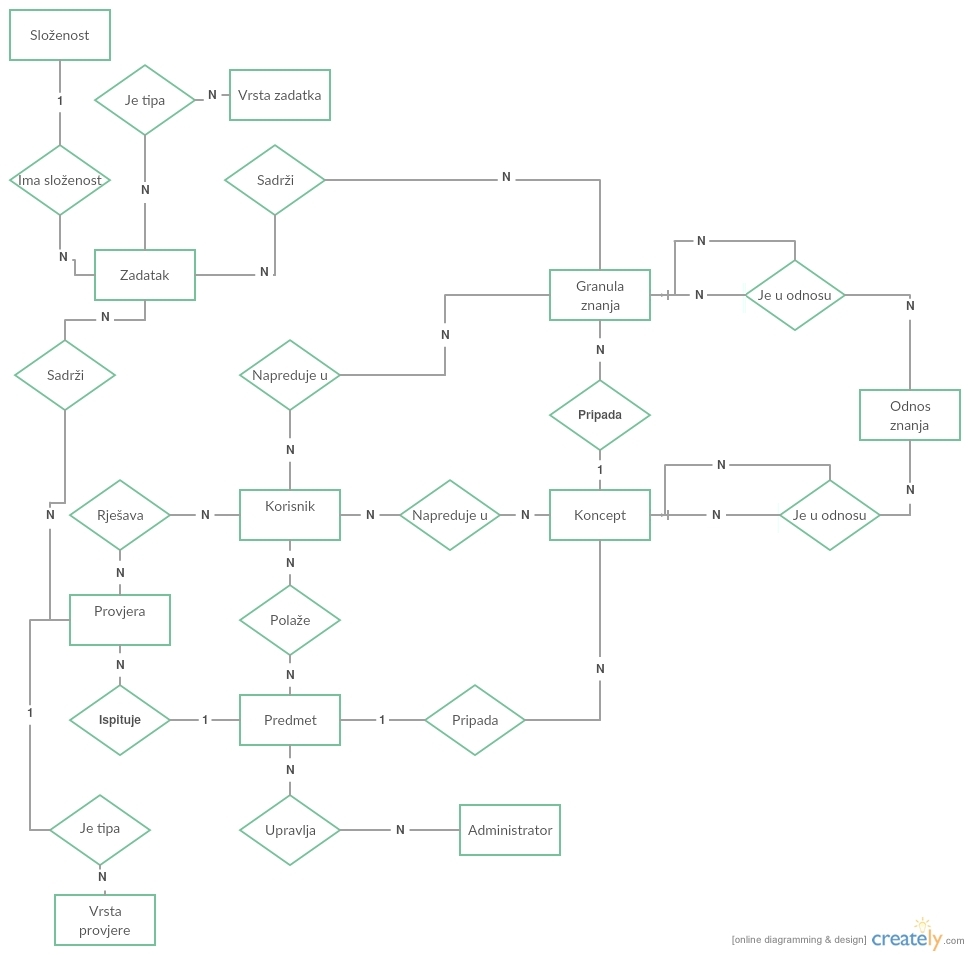
\includegraphics[width=\textwidth,height=\textheight,keepaspectratio]{img/ER.jpg}
	\caption{ER dijagram baze}
	\label{fig:ER}
\end{figure}
\begin{figure}[htb]
	\centering
	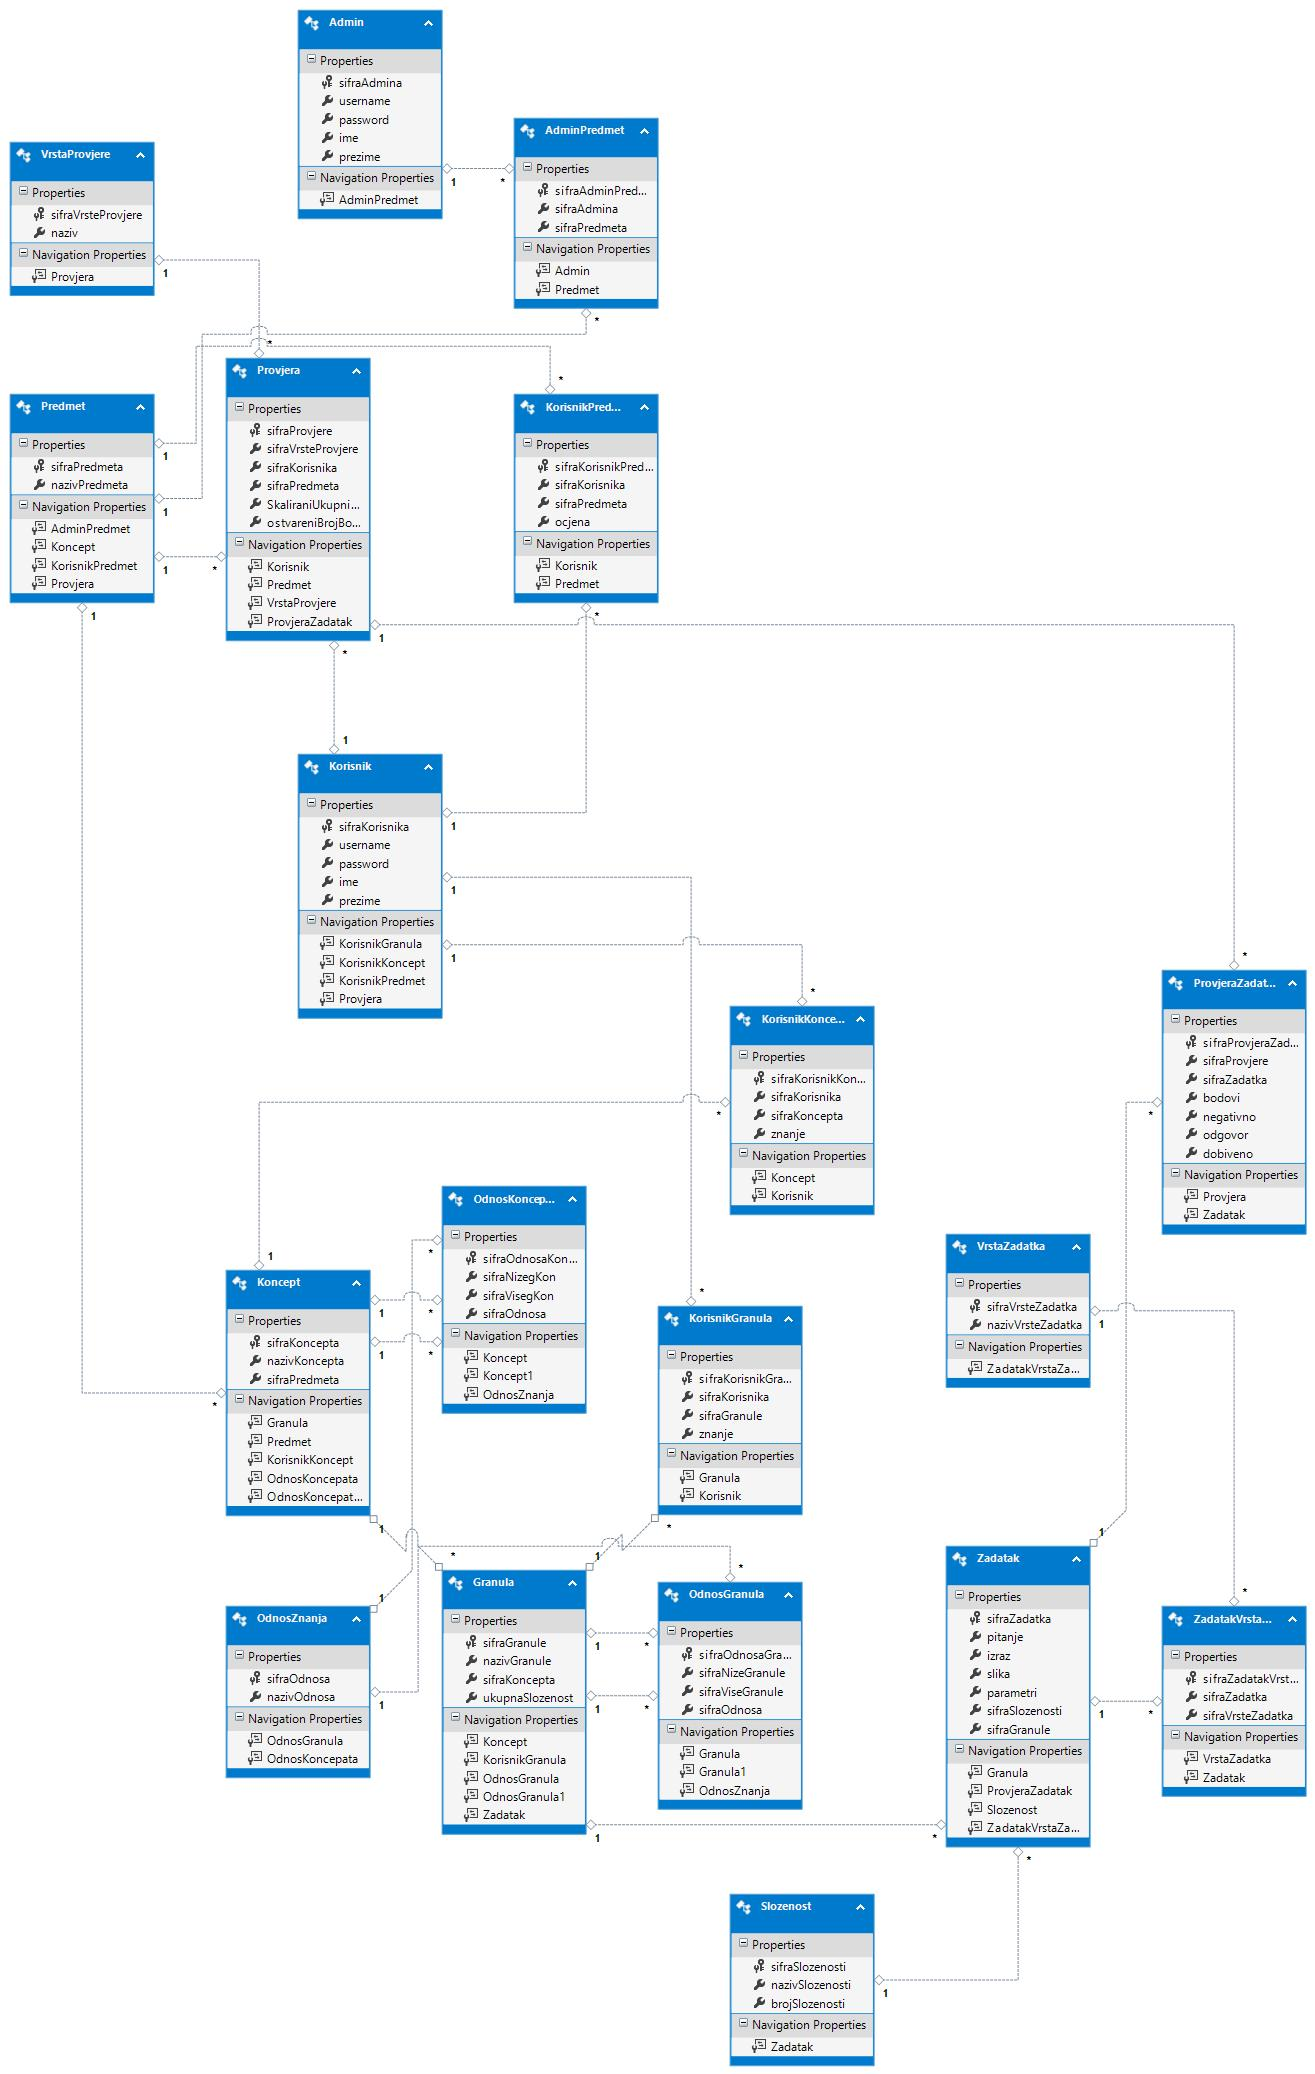
\includegraphics[width=\textwidth,height=\textheight,keepaspectratio]{img/dijagramEntiteta.jpg}
	\caption{Dijagram entiteta u bazi}
	\label{fig:dijagramentiteta}
\end{figure}
\pagebreak
\section{Mogućnosti sustava}
Mogućnosti sustava podijeljene su na one administratora, korisnika koji uči i zajedničke mogućnosti. Za obje vrste korisnika važne su granulacije znanja i način parametrizacije zadataka, za administratora je važno kako će dodavati pitanja u sustav, generirati ispite korisnicima te pregledavati njihove rezultate, a za korisnika koji uči registracija na sustav, način inteligentnog učenja te pregled vlastitih rezultata.

\subsection{Reprezentacija znanja}
Drugo poglavlje ovog završnog rada između ostaloga iznosi tezu o važnosti kvalitetne granulacije znanja u sustavu za inteligentno učenje. Stoga je njoj bio posvećen velik dio planiranja implementacije sustava. 

\subsubsection{Granulacije znanja}
Znanje se u ovom ITS-u dijeli na 3 kategorije: predmet, koncept i granula znanja.
\par 
Predmet je najveća kategorija te reprezentira sličnu količinu znanja kao jedan fakultetski kolegij, iako to nije nužno ukoliko se sustav ne koristi u svrhu formalne provjere. Entitet predmet je logičan početak zbog činjenice da sustav može biti korišten u svrhu različitih domena primjena s računskom osnovom te zbog toga da je jednostavno prirodan kao početna točka razmišljanja. Svaki predmet može imati svoje administratore koji mogu pregledavati rezultate, generirati testove i sl.
\par
Entitet predmet sadrži pripadne koncepte, a oni mogu pripadati samo jednom predmetu (1..N). Koncept je veća cjelina unutar predmeta koja se u dobro strukturiranim fakultetskim kolegijima može definirati kao jedan tjedan predavanja. Jedan predmet bi trebao sadržavati najmanje tri, a najviše 10-tak koncepata. Ne postoji konkretna preporučena brojka zato što svaki od predmeta može biti drukčije logički strukturiran.
\par
Svaki od koncepata sadrži granule znanja, najmanje granulacije ovog sustava. Granule znanja namijenjene su prikazivati neke specifične postupke, manje dijelove većih pojmova ili bilo koje druge nedjeljive cjeline čije se značenje pojavljuje u pojedinim zadacima. Također su vezane 1..N vezom, eksplicitno s konceptom, a time implicitno i s predmetom.
\pagebreak
\par
Primjer koji neće biti odrađen u ovom završnom radu, a mogao bi pomoći razumijevanju predviđene strukture podjele:
\begin{itemize}
	\item Predmet: Umjetna inteligencija
	\begin{itemize}
		\item Koncept: Pretraživanje prostora stanja
		\begin{itemize}
			\item Granula znanja: Pretraživanje u dubinu
			\item Granula znanja: Pretraživanje u širinu
			\item Granula znanja: A-zvjezdica pretraživanje
		\end{itemize}
		\item Koncept: Igranje igara
		\begin{itemize}
			\item Granula znanja: Minimax algoritam
			\item Granula znanja: Minimax s podrezivanjem
		\end{itemize}
	\end{itemize}
	\item Predmet: Osnove elektrotehnike
	\begin{itemize}
		\item Koncept: Magnetizam
		\begin{itemize}
			\item Granula znanja: Coulombova jednadžba
			\item Granula znanja: Naboji u prostoru
			\item Granula znanja: Dielektrici
		\end{itemize}
		\item Koncept: Istosmjerna struja
		\begin{itemize}
			\item Granula znanja: Strujni i naponski izvori
			\item Granula znanja: Kirchhoffovi zakoni
			\item Granula znanja: Načelo superpozicije
		\end{itemize}
	\end{itemize}
\end{itemize}

\subsubsection{Odnosi između granulacija}
Prilično je očito da samo tri granulacije znanja nisu dovoljne za opis svih mogućih situacija u znanju. Ukoliko dva različita predmeta imaju povezane koncepte (npr. Fourierova transformacija u MAT3 i SIS koji su dio 2. godine FER2 programa) želimo omogućiti da administratori predmeta mogu zabilježiti prethodno korisnikovo znanje. Ili unutar jednog predmeta, ponekad nema smisla korisnika dvaput ispitivati analogne stvari (npr. osnove Theveninovog teorema za izmjeničnu i istosmjernu struju). Ili jednostavno želimo korisniku onemogućiti da otvara neke nove koncepte prije dokazivanja prihvatljive razine znanja u prethodnima (npr. korisnika koji ne poznaje kombinatoriku nema smisla ispitivati pitanja iz diskretne vjerojatnosti). Stoga ovaj sustav donosi dodatnu mogućnost modeliranja znanja: odnose između granulacija.
\par
Odnosi mogu biti definirani samo između dvije granulacije jednake vrste i to samo za koncepte i granule znanja. Definicija na razini predmeta nije potrebna zato što je predmet "sačinjen" od koncepata, a nema ograničenja u pogledu odnosa koncepata dvaju različitih predmeta. U sustavu su definirani sljedeći odnosi:

\begin{itemize}
\item \textbf{Preduvjet} Ovaj odnos definira nemogućnost otvaranja sljedeće granulacije prije postizanja prihvatljive razine znanja u baznoj. Prihvatljiva razina znanja ekvivalent je ocjene dovoljan na pojedinoj granulaciji.

\item \textbf{Podskup (nadskup)} Odnos između dvije granulacije u kojom je jedna u potpunosti sačinjena od druge. Podrazumijeva se da je niža granulacija pravi podskup jer semantički nema smisla imati dvije identične granulacije, iako to sustav nigdje eksplicitno ne provjerava.
\item \textbf{Korištenje} Ukoliko je znanje definirano nekom granulacijom uvijek nužno koristiti u drugoj, nema potrebe za stalnim eksplicitnim povezivanjem zadatka i te granulacije nego administrator može zadati odnos korištenja.
\item \textbf{Analogno} U situacijama u kojima postoji jasna povezanost između dvaju pojmova, takva da znanjem jednog postoji razumijevanje drugog, može se definirati ovaj odnos. U takvom slučaju korisniku se dodaju male količine znanja analognog pojma te postoji mogućnost za manjim brojem elementarnih pitanja u početku ispitivanja novog pojma.
\item \textbf{Paralelno} Postoji mogućnost da dvije granulacije opisuju istu situaciju na različite načine (npr. pristupi umjetnoj inteligenciji - logički, kognitivni, itd.) te zapravo korisnik uči više različitih pogleda. Za logiku sustava i model učenja paralelnost granulacija znanja nema nikakvog utjecaja te je ona tu samo da korisnik bolje razumije što i kako uči. 
\end{itemize}

Niti jedan od odnosa ne isključuje korištenje bilo koje drugog, no preporuka autoru pitanja je da ne pretjeruje s kombiniranjem više od dva-tri odnosa po jedinki granulacije da sustav ne bi zapetljao tako da eliminira inteligentno posluživanje pitanja.

\subsection{Parametrizirani zadaci}
Jedan od zadataka ovog završnog rada je parametrizacija pitanja koja se poslužuju korisniku. Ona je izvedena na razinama baze podataka i aplikacijske logike. Izrazi su zapisani u bazi podataka, a konkretne parametre generira aplikacijska logika.

\subsubsection{Zapis u bazi podataka i generiranje}
Svako pitanje u bazi predstavljeno je entitetom zadatak koji sadrži tekstualno pitanje, matematički izraz koji treba izračunati, eventualno sliku te parametre. Parametri trebaju biti zapisani u standardnom tekstualnom obliku: "parametar:uvjet parametar:uvjet", itd. Član parametar predstavlja samo ime tog parametra, a uvjet činjenicu da mora biti veći ili manji od nekog broja. Standardan zapis uvjeta je: >broj1\&<broj2. Ukoliko parametar nema uvjeta, zapisuje se "none". Vrijednosti parametara koje se zadaju pojedinom korisniku generira sustav i one mogu biti isključivo decimalne.
\par
Parametre uz poštovanje uvjeta generira aplikacijska logika. Parametri su decimalni brojevi predodređenog raspona između atributa minParametar i maxParametar koji su trenutno postavljeni na 0 i 120. Svaki parametar može odrediti svoju domenu uvjetima, a niti jedan od parametara trenutno sadržanih zadataka ne nalazi se izvan tog skupa. Jedina svrha tih dvaju atributa je optimizacija jer nema smisla generirati parametre koji nikada neće zadovoljavati uvjete pitanja.

\subsubsection{Izračun rezultata}
Nakon što je korisniku predstavljena vrijednost parametara i on odgovori na pitanje, na temelju tih vrijednosti sustav izračuna predviđeni odgovor te s tolerancijom od 5 posto uspoređuje njegov i predviđeni odgovor. Izračun se izvodi uz pomoć mXparser biblioteke.

\subsection{Mogućnosti administratora}
U sustavu postoji veza između predmeta i administratora koja znači da samo na određenom predmetu sljedeće operacije mogu raditi samo oni administratori koji imaju ovlasti. To je logično kod svakog većeg sustava, no ipak je važno i eksplicitno napomenuti.

\subsubsection{Registracija korisnika na predmet}
Prilikom registracije korisnika u sustav, on nije povezan s predmetima, već ga administrator mora dodati na predmet kojim upravlja. On ne može izbrisati korisnika sa predmeta, tj. učiniti kao da nikada nije postojao, već mu samo dati negativnu zaključnu ocjenu.

\subsubsection{Generiranje ispita}
Administrator na svojem predmetu ima mogućnost generiranja ispita za zadane korisnike. Ispitu se zadaje broj bodova, broj zadataka i faktor složenosti između 1 i 5. Faktor složenosti određuje prosječnu složenost zadataka na ispitu. Moguće je zadati i maksimalnu/minimalnu složenost zadataka na ispitu ako administrator želi imati veću kontrolu nad generiranjem ispita.
Ukoliko sustav nema dovoljno pitanja s takvim parametrima o tome obavještava administratora te čeka ili dozvolu generiranja ispita manjeg broja zadataka ili unos novih parametara za generiranje.
Administrator nema mogućnost određivanja bodovanja pojedinog zadatka zbog inteligencije sustava koja sama određuje najbolje bodovanje. Na to administrator može utjecati samo prilikom zapisivanja pitanja u bazu biranjem njegove složenosti.
Ispit mora biti generiran za određene korisnike sudionike na pojedinom predmetu. Ukoliko sustav shvati da korisnicima ne bi smjela biti ponuđena pitanja s parametrima koje je odredio administrator (tj. neki od korisnika nisu zadovoljili preduvjete), sustav nudi mogućnost poništenja generacije ispita ili nastavak. Pretpostavka je da je administrator možda pogriješio ili da korisnik nije bio dovoljno odgovoran u rješavanju zadataka.

\subsubsection{Pregled rezultata}
Administrator može vidjeti rezultate korisnika na svome predmetu, a oni uključuju: pregled korisnikova znanja na pojedinoj provjeri, korisnikovo znanje na pojedinom konceptu tog predmeta te preporučenu konačnu ocjenu za navedeni predmet.
Ukoliko administrator odluči potvrditi tu ocjenu, korisniku se zaključava navedeni predmet i u sustav zapisuje konačna ocjena.

\subsection{Mogućnosti korisnika}
Sljedeće mogućnosti korisnici mogu odgovarati samo na pitanja iz predmeta kojima pripadaju, baš kao i administratori. Za registraciju na pojedini predmet korisnici koji uče moraju čekati odobrenje administratora.

\subsubsection{Registracija}
Novi korisnici koji žele učiti mogu se registrirati na sustav te od administratora predmeta zatražiti pristupanje nekom predmetu. Nakon uspješne registracije korisnika i dodavanja predmeta, korisnik odmah može započeti proces učenja. Lozinku korisnika sustav sprema na siguran način posoljenim hash SHA256 algoritmom, kao što se očekuje od svakog ozbiljnog ITS-a.

\subsubsection{Inteligentno učenje}
Svi korisnici učenje počinju od samog početka što znači da ne postoji mogućnost prenošenja rezultata iz nekog drugog ITS-a. Korisniku se nudi inteligentno učenje na pojedinom predmetu, tj. mogu se generirati samo ona pitanja čije su granule znanja povezane s konceptima točno određenog predmeta. No, odgovaranje na pitanja jednog predmeta može dovesti i do promjene stanja na drugom predmetu u slučaju da je baza znanja koncipirana tako da su koncepti ili granule znanja jednog predmeta u odnosu s onima drugog.
\par
Bit inteligentnog učenja je u praćenju korisnikova znanja i odabiru pitanja što se ponajprije očituje u tome da korisniku sustav ne smije postavljati pitanja na koja još ni u kojem slučaju ne može  znati odgovor. Zbog toga su vrlo važni složenost pitanja i odnos preduvjeta. No, o konkretnom načinu posluživanja pitanja bit će riječi u sljedećem poglavlju.
\par
Korisnici mogu pisati dvije vrste provjere: vježbe i ispite. Vježbe su provjere kojima se ostvaruje napredak u sustavu na kojima korisnik može više puta griješiti bez dugoročnih posljedica po konačnu ocjenu iz predmeta. Od korisnika se očekuje da stalno otvara vježbe, uspješno napreduje te kad se osjeća sigurnim, zatraži generiranje ispita za određeni predmet. Prvi ispit ne znači završavanje ili padanje predmeta, znači samo to da se njegovi bodovi pamte. Sam sustav određuje koja su pitanja najprikladnija za nekog korisnika na pojedinom predmetu. 
\par
Ispiti su formalne provjere kojima se polažu predmeti. Generiranje ispita zadaje administrator ili traži korisnik. Korisnik sve teoretski može polagati putem ispita, no to nema previše smisla zato što u reprezentaciji znanja nema veće koristi u rješavanju ispita, oni su tu samo za formalno određivanje ocjene. Ispiti koje traži korisnik također se generiraju putem algoritma za inteligentno učenje. Za reprezentaciju korisnikova znanja nema razlike u odgovaranju na isto pitanje u vježbi i ispitu.

\subsubsection{Pregled rezultata}
U svakom trenutku izvan odgovaranja na provjeru, korisnik može pogledati svoje rezultate na nekom predmetu. Mogu mu se ispisati detalji provjera kojima je pristupio (ne i konkretna pitanja koja je na njima vidio), trenutna predviđena ocjena na tom predmetu i prikaz znanja po konceptima tog predmeta.
\par
Osim svojih rezultata korisnik može vidjeti i sve granule znanja pojedinog koncepta na predmetu te veze koje taj koncept ima.

\section{Procjena znanja korisnika}
Algoritam procjene znanja radi u dva koraka, najprije procjenjuje znanje pojedinih granula, a zatim na temelju te procjene procjenjuje znanje koncepata. Algoritam se aktivira nakon što korisnik završi rješavanje provjere. Ako se tijekom vježbe ili ispita dogodi neočekivani prekid rada aplikacije, korisnikovo znanje granula i koncepata ostaje isto kao prije generiranja, no na ispitima to znači da je korisnik osvojio 0 bodova.

\subsection{Procjena za granule znanja}
Procjena usvojenosti znanja granula temelji se na vezi zadatka i granule, složenosti zadatka i odnosima između granula. Točno odgovoreni zadatak korisnikovom znanju pojedine granule dodaje broj složenosti tog zadatka. Npr. prvim odgovaranjem na osnovno pitanje iz nekog pojma koje ima broj složenosti 1, korisnikovo znanje granule se povećava s 0 na 1. Ako je odgovor netočan, korisnikovo znanje smanjuje se za isti broj, tj. u ovom primjeru bilo bi -1.
\par
Nakon dodavanja znanja osnovnoj granuli zadataka algoritam iterativno prolazi po svim odnosima te granule na sljedeći način:
\begin{itemize}
	\item Ako je granula podskup neke druge granule, granuli koja je sadrži se na jednak način dodaje točnost/netočnost odgovora.
	\item Ako granula koristi neku drugu prilikom rješavanja zadatka (npr. diskretnu vjerojatnost je nemoguće izračunati bez poznavanja osnova kombinatorike), korištenoj granuli dodaje se ili oduzima faktorKorištenja*složenost. Trenutni faktor korištenja postavljen je na 0.4, no postoji mogućnost promjene temeljem iskustva (promjena nije automatizirana).
	\item Ako postoji granula čije je znanje analogno znanju trenutne granule, korisnikovo znanje analogne granule mijenjamo za faktorAnalognosti*složenost. Trenutni faktor analognosti je 0.2. Valja naglasiti da analognost nije dvosmjerna, tj. ako administrator želi dvosmjernu analognost, u bazi mora postaviti da je X analogno s Y i Y analogno s X.
\end{itemize}

Granule u bazi sadrže atribut ukupna složenost koji se računa kao suma složenosti zadataka te granule + ukupna složenost granula koje su njezini podskupovi.

\subsubsection{Prednosti ovakvog pristupa}
Razlozi za ovakav pristup procjeni znanja granula su: trajnost znanja, inkrementalni pristup i brzina izračuna.
\par
Trajnost znanja očituje se u tome da jedna pogreška u sustavu znači manje nego višestruki broj točnih odgovora, no istovremeno znači da se korisnika koji ne zna odgovoriti na teža pitanja, vraća na lakša. Znanje korisnika mapira se od minimalnog do maksimalnog \textit{double} broja.
\par
Inkrementalni pristup očituje se u algoritmu odabira pitanja koji procjenuje složenost trenutnog znanja korisnika te na temelju nje poslužuje pitanja najbliže složenosti. Nakon što korisnik odgovori na ta pitanja, točni odgovori povećavaju njegovo znanje te se nude pitanja više složenosti, a netočni odgovori ga vraćaju na nižu razinu (uz uvjet da je odgovorio na dovoljan broj pitanja jedne granule).
\par
Brzina izračuna nije bila presudni faktor projektiranja baš ovakvog algoritma, no ipak je izuzetno važno da sustavu ne treba previše vremena za aktualizaciju pa je ona ugodna nuspojava ovog pristupa.

\subsection{Procjena za koncepte}
Procjena znanja za koncepte slijedi tek nakon procjene znanja granula. Ona se računa na sljedeći način:
1. Za sve granule koje pripadaju konceptu računa se postotak usvojenosti.
2. Za granule koncepata koji su u odnosu s trenutnim također se računa postotak usvojenosti.
3. Izračunava se težinski prosjek postotaka usvojenosti sljedećom formulom:
\begin{center}
	U = $\sum_{i=1}^{n} T\textsubscript{i}*G\textsubscript{i}$ / $\sum_{i=1}^{n} T\textsubscript{i}$
\end{center}
U - postotak usvojenosti, n = ukupni broj granula iz 1. i 2. korak, T\textsubscript{i} = težina, G\textsubscript{i} - postotak usvojenosti i-te granule.
Težine pojedinih granula su:
\begin{itemize}
	\item T = faktorVažnosti ako granula pripada trenutnom konceptu ili konceptu koji je podskup trenutnog.
	\item T = faktorKorištenja*faktorVažnosti ako koncept koristi neki drugi.
	\item T = faktorAnalognosti*faktorVažnosti ako je koncept analogan nekom drugom konceptu
\end{itemize}
Trenutni faktor važnosti postavljen je na 5.

\subsubsection{Prednosti ovakvog pristupa}
Dvije najbitnije prednosti ovakvog pristupa su razumljivost prikaza i sigurnost točnog izračuna. Razumljivost prikaza napretka korisnika samom korisniku vrlo je značajna za točnu predstavku o vlastitome znanju. Postotni prikaz razumiju gotovo svi te je relevatniji od možda nepreglednih dijagrama. Težinskim prosjekom korisnik je lišen razmišljanja o implementacijskim detaljima odnosa koncepata u prikazu njegova znanja, no on te odnose može vidjeti ako želi.
Sigurnost točnog izračuna postiže se izračunom znanja iz granula, a ne prijašnjih rezultata koncepata. Kada bi se znanje računalo i na razini granula znanja i na razini koncepata, postoji mogućnost previše međuovisnosti i pogrešnog izračuna.

\subsection{Ocjena za predmete}
Ocjene za predmete određuju se zbrajanjem ostvarenih bodova korisnika na svim ispitima te dijeljenjem tog broja s ukupnim mogućim brojem bodova.
Ocjene su definirane sljedećim pragovima:
\newline
<50\%: 1, 
50\% - 60\%: 2, 
60\% - 70\%: 3, 
70\% - 85\%: 4, 
>85\%: 5

\section{Logika posluživanja pitanja}
Logika posluživanja pitanja vrlo je važan dio ovog sustava, a slijedi dva principa:
1. Korisniku treba poslužiti pitanja koja će mu predstavljati rješivi izazov, tj. ne treba mu nuditi pitanja koja je već dokazano točno riješio niti pitanja koja ne može odgovoriti temeljem trenutnog znanja
2. Svaka provjera treba sadržavati što veći broj različitih pitanja (osim ako drukčije ne postavi administrator) da ne bi naučio "kuharicu" i umjetno preskočio neke dijelove ili ako korisnik nešto ne zna, nema smisla ponuditi mu provjeru ispunjenu pitanjima te vrste.

\subsection{Algoritam posluživanja pitanja}
Logika posluživanja pitanja unutar ovog sustava zapravo je vrlo jednostavna i prikazana je sljedećim algoritmom:
\newline
1. Dohvati sve koncepte unutar predmeta koje korisnik može odgovarati (zadovoljio je preduvjete ili preduvjeti ne postoje).
\newline
2. Za svaki od koncepata uzmi dostupne granule, permutiraj listu svih granula.
\newline
3. Za svaku od granula uzmi po jedno pitanje prema 6. koraku.
\newline
4. Ponavljaj 3. korak dok ne ispuniš broj pitanja. Ako nema dovoljno pitanja, uzimaj po dva pitanja za svaku od granula.
\newline
5. Ponavljaj 4. korak dok se ne ispuni uvjet prekida povećavajući broj pitanja koji se uzima za jedan. Ako su sve kombinacije pitanja iskorištene, prekini traženje i ponudi manji broj pitanja unutar provjere.
\newline
6. Pitanja uzimaj po principu:
\newline
a) aproksimiraj prosječnu složenost znanja korisnika za neku granulu.
\newline
b) nađi pitanje s najbližom složenošću koje nije već uzeto za  ovu provjeru.
\newline
7. Nakon završetka odabira pitanja, generiraj konkretnu provjeru sa konkretnim pitanjima.

\section{Konkretna pitanja u sustavu}
Pitanja unutar sustava pitanja su jednog zamišljenog predmeta - diskretne matematike, a njegovo je znanje dio dvaju predmeta na Fakultetu Elektrotehnike i Računarstva - Matematike 3R i Vjerojatnosti i statistike. Niti jedan od tih stvarnih predmeta nije u cijelosti sadržan unutar ovog sustava, on sadrži samo dijelove vezane uz diskretnu matematiku. Inspiracija za tekstualni opis preuzeta je iz udžbenika \cite{zubrinic} i \cite{elezovic}, no tamošnja sadržavaju konkretne brojke, a ovaj sustav sadrži formulama generalizirane verzije.

\subsection{Test točnosti parametrizacije}
Generiranje parametara i računanje rezultata testirano je na 10.000 različitih kombinacija parametara za pojedino pitanje te ta mogućnost i dalje postoji u sustavu. Tu se izuzetno korisnim pokazalo svojstvo mXparsera da svaku pogrešku u svom radu vraća kao NaN (nepostojeći broj) umjesto da baca grešku. Sve uočene pogreške riješene su te bi sustav generiranja parametara trebao raditi u potpunosti.

\pagebreak
\subsection{Znanje u sustavu}
\begin{itemize}
	\item Predmet: Diskretna matematika
	\begin{itemize}
		\item Koncept: Osnove kombinatorike
		\begin{itemize}
			\item Granula znanja: Skupovi
			\item Granula znanja: Produktno pravilo
			\newline - nadskup: skupovi
			\item Granula znanja: Permutacije
		\end{itemize}
		\item Koncept: Varijacije - paralelno: kombinacije
		\begin{itemize}
			\item Granula znanja: Varijacije s ponavljanjem
			\item Granula znanja: Varijacije bez ponavljanja
		\end{itemize}
		\item Koncept: Kombinacije - paralelno: varijacije
		\begin{itemize}
			\item Granula znanja: Kombinacije s ponavljanjem
			\item Granula znanja: Kombinacije bez ponavljanja
		\end{itemize}
		\item Koncept: Napredna kombinatorika
		\newline - nadskup i preduvjet: osnove komb., varijacije, kombinacije
		\begin{itemize}
			\item Granula znanja: Mješovita kombinatorika
			\item Granula znanja: Teorija grafova
		\end{itemize}
		\item Koncept: Osnove diskretne vjerojatnosti
		\newline - preduvjet: osnove kombinatorike
		\begin{itemize}
			\item Granula znanja: Klasični vjerojatnosni prostor
			\item Granula znanja: Beskonačni vjerojatnosni prostor
			\item Granula znanja: Geometrijske vjerojatnosti
			\newline - analogno: produktno pravilo
		\end{itemize}
	\end{itemize}
\end{itemize}

\chapter{Zaključak}
Edukacijski procesi značajan su i vrlo složen element ljudske civilizacije, a razvojem tehnologije i otklonom od manualnih djelatnosti, njihova važnost još više raste. Stoga je neizbježna potreba za unaprjeđenjem, olakšanjem i poboljšanjem procesa učenja, pogotovo u modernom svijetu u kojem je vrijeme pažnje čovjeka sve kraće.
\par
Sustavi za inteligentno učenje (ITS) nameću se kao logično moguće rješenje novih izazova, a također istovremeno smanjuju povezanost fizičke pozicije ljudi i njihovog znanja. Internet je danas dostupan gotovo svuda te su sustavi za inteligentno učenje konačno dobili platformu širenja.
\par 
No, da bi sustav za učenje bio kvalitetan mora imati razrađenu podjelu znanja u manje granulacije i praćenje korisnikova znanja, pitanja u njemu moraju biti parametrizirana, mora biti (relativno) siguran za korištenje te biti izrađen kao skup tipičnih komponenti. Te komponente su domenski model, korisnički model, model učenja i korisničko sučelje. Jedini od modela koji može nedostajati je korisnički model, ako je njegova funkcionalnost rastavljena u domenski i model učenja. Kako bi taj sustav još bio i inteligentan, nužno je da ima iznimno dobro razrađeno praćenja korisnikova znanja te algoritme posluživanja pitanja. Pravi  komercijalni inteligentni sustavi još mogu i pratiti tipkanje i facijalne reakcije korisnika te imati prilagođene upute za korisnika koji ih zatraži.
\par
Iako sustavi za učenje na prvi pogled djeluju kao isključivo pitalice s odgovorima, to u praksi nije baš tako, dapače, svaki sustav koji ima edukacijsku svrhu, a nema oblik pitalice je korak unaprijed za proces učenja. Neki od takvih sustava su edukativna igra Urban Jungle, sustav koji vokalno razgovara s korisnikov AutoTutor te Why2-Atlas koji komunikaciju izvodi tekstualno.
\par
ITS je sigurno kvalitetan i zanimljiv koncept, no i on sadrži neke nedostatke, ponajprije inteligenciju ograničenu znanjem autora, nužnost kvalitetne interdisciplinarne suradnje te visoku cijenu izrade.
\par
Posljednji dio ovog završnog rada prikazao je dizajn jednog vlastitog sustava za inteligentno učenje s parametriziranim pitanjima, reprezentacijom znanja različitim granulacijama, inteligentnim posluživanjem pitanja, ali i administratorskim nadzorom. Takva implementacija relativno je jednostavna u odnosu na komercijalne sustave, no ona je ITS.
\par
Nakon podužeg vremena zapostavljanja sustava za (inteligentno) učenje u odnosu na ostale primjene umjetne inteligencije, sada se sa sigurnošću može tvrditi da oni konačno imaju veliku mogućnost razvoja te mnoge stvarne primjene.

\bibliography{literatura}
\bibliographystyle{fer}

\begin{sazetak}
Ovaj završni rad opisuje modernizaciju procesa učenja sustavom za inteligentno učenje. Rad počinje uvodom u edukacijske procese, zatim prikazuje povijest ideje automatizacije učenja te suvremeni model sustava za inteligentno učenje (ITS). ITS je opisan svojim komponentama, očekivanim karakteristikama i algoritmima uz kritički pogled na nedostatke ITS-a. Slijedi opis slojeva aplikacije koje je potrebno implementirati te opis implementiranog rješenja. On sadrži popis korištenih tehnologija, ER dijagram baze te mogućnosti koje sustav nudi korisniku koji uči te administratoru. Opis završava logikom posluživanja pitanja. Posljednje poglavlje rada je zaključak o prethodno iznesenim idejama. 

\kljucnerijeci{Učenje, inteligentno učenje, informacijski sustav, ITS, znanje, prikaz znanja, parametrizacija, posluživanje pitanja, podatkovni sloj, aplikacijski sloj}
\end{sazetak}


\engtitle{Application logic and data layer development for an e-learning system}
\begin{abstract}
This paper describes modernization of the learning processes using intelligent tutoring system. It begins with introduction  to educational processes, it then describes the history of automated	 learning and contemporary model of an intelligent tutoring system (ITS). The paper then describes layers of the application to be implemented and the implemented solution. This description contains a list of used technologies, ER diagram of the database and all options the system offers to both learning user and an administrator. It is followed by the description of the logic of serving questions. The last chapter is a conclusion about aforementioned ideas.

\keywords{Learning, intelligent learning, information system, ITS, knowledge, knowledge representation, parameterization,  question serving, data layer, application logic}
\end{abstract}

\end{document}